\documentclass[10pt,a4paper]{article}
\usepackage[utf8]{inputenc}
\usepackage[T1]{fontenc}
\usepackage[spanish]{babel}
\usepackage{amsmath}
\usepackage{amsfonts}
\usepackage{amssymb}
\usepackage{graphicx}
\usepackage{float}
\usepackage{lipsum}
\usepackage{multicol}
\usepackage{xcolor}
\addto{\captionsspanish}{\renewcommand{\abstractname}{Abstract}}
\newcommand{\celda}[1]{
	\begin{minipage}{2cm}
		\vspace{2mm}
		#1
		\vspace{2mm}
	\end{minipage}
}
\definecolor{azul}{rgb}{0.36, 0.54, 0.66}
\usepackage[left=2.00cm, right=2.00cm, top=2.00cm, bottom=2.00cm]{geometry}
\author{Gabriel Hernandez Bello}
\begin{document}
	
	\begin{figure}[H]
		\raggedright
		
\includegraphics[scale=0.2]{IMG/logo_udec.png} \hfill 
\includegraphics[scale=0.5]{IMG/cfm_logo.png}
	\end{figure}

	\vspace{6mm}
	%ESTE CENTER ES EXCLUSIVO PARA EL TITULO DEL PAPER, AUTOR Y UNIVER.
	\begin{center}
		{\Large \textbf{Medición de la altura del Campanil}}\\
		\vspace{2mm}
		{\large Gabriel Hernández Bello$^{1}$}\\
		\vspace{6.5mm}
		$^1$\textit{Universidad de Concepción, Facultad de Ciencias Físicas y Matemáticas, Ciencias Físicas. }\\
	\end{center}

	\begin{center}
		\textcolor{azul}{\rule{150mm}{0.8mm}}
	\end{center}

      %ESTE ABSTRACT ES PARA EL RESUMEN PROPIAMENTE DICHO Y PARA LAS PALABRAS CLAVES (KEYWORDS) ,NOTA:el comando \par sirve para iniciar el nuevo parrafo con sangría.
	\begin{abstract}
		\underline{\textbf{Palabras Claves:}} \hspace{2mm} \textit{palabra1, palabra2, palabra3.}
	\end{abstract}
	
	\begin{center}
		\textcolor{azul}{\rule{150mm}{0.8mm}}
	\end{center}
	
	\begin{multicols}{2}
		\section*{Introducción} \label{Intro}
			El campanil de la Universidad de Concepción es un campanario icónico de la universidad y la ciudad chilena de Concepción \cite{wikicamp}. Fue construido hacia 1943 gracias a la iniciativa de Enrique Molina Garmendia, quien apasionado por la Universidad de California, en Berkeley, esgrimía la idea de una \emph{ciudad universitaria} abierta para todos los visitantes y en la que se levantara un imponente campanil. El proyecto del campanil fue elegido del arquitecto Enrique San Martín y posteriormente construido bajo la suérvisión del Constructor Civil Juan Villa Luco. Se hizo de concreto armado, con 42 metros y 50 centímetros de altura, con escaleras en su interior y un balcón en la parte superior.\\
			En el presente laboratorio, usaremos herramientas matemáticas para calcular y verificar la altura del Campanil de la Universidad de Concepción.
		\section*{Marco Teórico} \label{marco}
		\subsection*{Trigonometría}
		La trigonometría es una rama de la matemática que se encarga de estudiar y medir los triángulos, las relaciones entre sus ángulos y lados, y las razones trigonométricas. Estas son de gran interés por su amplia aplicabilidad.\\
		Las razones entre los lados de un triángulo rectángulo son llamadas trigonométricas. Las principales son el \emph{seno, coseno} y la \emph{tangente}.\\
		\section*{Procedimiento Experimental y Resultados}
		Para calcular la altura del Campanil, diseñamos un instrumento sencillo para medir ángulos, compuesto por un transportador, una regla, un hilo y un objeto pesado. De esta forma, apuntamos el instrumento hacia la cima del Campanil, lo que provoca que el hilo (tensado por el peso) se desplace de su posición de equilibrio, formando un ángulo que medimos con el transportador. Además, usamos una hunicha para medir la separación entre el Campanil y la posción donde se mide el ángulo. Luego, estimamos la altura del Campanil para distintas distancias usando la siguiente fórmula:
		\begin{equation}
		D = d + L \tan(\alpha).
		\end{equation}
		Donde $D$ representa la altura del campanil, $L$ la distancia entre campanil y el punto de medición del ángulo, $d$ la distancia entre la base del campanil y el punto de observación del ángulo y $\alpha$ el ángulo obtenido con el instrumento de medición.
		
		
		\begin{figure}[H]
			\centering
			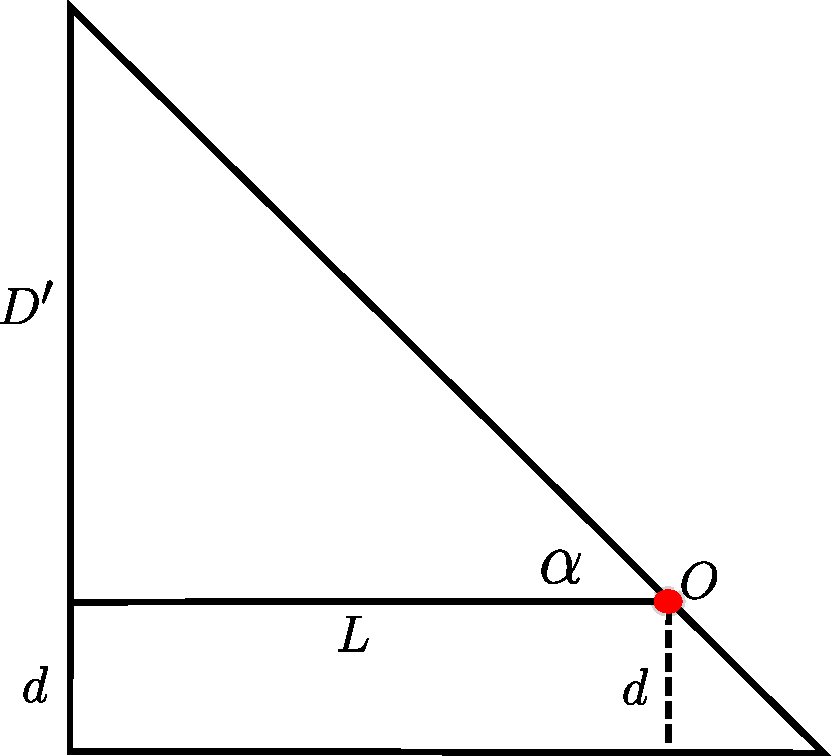
\includegraphics[scale=0.4]{IMG/camp.pdf} 
			\label{grafico campanil}
			\caption{Diagrama de la medición de la altura del campanil. Se respresenta $D^{\prime} = L \tan(\alpha)$,  $d$ la altura desde la base hasta el punto de observación del ángulo $O$ y $L$ la distancia entre el campanil y el punto de medición del ángulo.}
		\end{figure}
		
	En la siguiente tabla \ref{tabla valores} se recogen los datos obtenidos para tres distancias y ángulos diferentes:
	\end{multicols}
	
	\begin{table}[H]\label{tabla valores}
	\centering
\begin{tabular}{|c|c|c|c|}
\hline
\textbf{$\alpha$ (°)} & $L$ (m) & $d$ (m)&  $D$ (m) \\ \hline
35.0 $\pm$ 0.5  & 56.3000 $\pm$ 0.0005 &  1.6000 $\pm$ 0.0005 & 41.02 \\ 
40.0 $\pm$ 0.5 & 50.0000 $\pm$ 0.0005 & 1.6000 $\pm$ 0.0005 & 43.55 \\ 
45.0 $\pm$ 0.5 & 43.0000 $\pm$ 0.0005 & 1.6000 $\pm$ 0.0005 &  43.00 \\ \hline
\end{tabular}
\caption{Ángulos y Distancias Medidas}
\label{tab:angulos_distancias.}
\end{table}

\begin{multicols}{2}
Considerando el valor medio de la altura estimada $\bar{D}$, obtenemos $\bar{D} = 42.52$, con un error representado por la desviación estándar $\sigma_D = 0.94$. Por lo tanto, la altura del campanil determinada experimentalmente es $D = 42.52 \pm 0.94$.\\

\subsection*{Análisis}
La altura del Campanil de la Universidad de Concepción es un dato conocido. Por ello, es posible estimar el \emph{error absoluto} y el \emph{error relativo} de nuestra medida:
\begin{align}
\varepsilon_{abs} &= |D - \bar{D} | = 0.02. \\
\varepsilon_{rel} & = \frac{\varepsilon_{abs}}{\bar{D}} \cdot 100 =  0.05\%.
\end{align}
Ambos errores son prácticamente despreciables, por lo que válidamos tanto el proceso experimental como el tratamiento de las medidas obtenidas emipíricamente. 
\subsection*{Conlusión}
En el Análisis evidenciamos la efectividad del método empleado para estimar la altura del Campanil. Aunque las mediciones fueron realizadas con una rigurosidad relativa, obtuvimos resultados muy cercanos al valor esperado. Con ello, ponemos de manifiesto la gran capacidad y utilidad de las matemáticas utilizadas que, a pesar de su antigüedad, continúan siendo un recurso potente e indispensable para, por ejemplo, estimar la altura del campanil.


		
	\end{multicols}
	
	\bibliographystyle{unsrt}
	\bibliography{ref}

\end{document}